\chapter{Srovnání výsledků}

Odvozený model identifikovaný z rovnic v kapitole \ref{identifikovane_parametry_ch} dává do vztahu točivé momenty s polohami, úhlovými rychlostmi a úhlovými zrychleními na jednotlivých osách (rovnice \ref{celkova_dyn_rovnice_eq}). Tento model je dále možné použít k výpočtu celkového elektrického výkonu robota (viz sekce \ref{el_vykon_ch}).

Vypočítané momenty sil na jednotlivých osách se pomocí momentových konstant převedly na efektivní hodnoty proudů protékajících vinutími motorů. Nahrazením vinutí motorů obvodem s odporem a indukčností zapojenými v sérii byly z těchto hodnot proudů vypočítány jednotlivé hodnoty efektivního napětí na svorkách motorů. Vynásobením hodnot napětí a proudů byly vypočítány elektrické výkony na jednotlivých osách. Celkový elektrický výkon robota je poté dán součtem všech dílčích výkonů na všech osách. 

Pro porovnání modelu pro výpočet výkonu s reálnými naměřenými hodnotami byla použita jiná trajektorie, než která byla použita pro jeho identifikaci. Tato testovací trajektorie byla vytvořena tak, aby se co nejvíce blížila typickým trajektoriím vyskytujícím se v průmyslových aplikacích. Byla vybrána trajektorie simulující montáž součástky A na povrch součástky B. Koncový efektor robota nejprve dojel z výchozí pozice na pozici, kde by se měl vyskytovat zásobník se součástkou A. Poté koncový efektor po obloukové trajektorii dojel na místo montáže součástky A a natočil se do požadovaného úhlu. Následně se vrátil zpět do výchozí pozice.

Při tomto pohybu robota byl v řídícím systému robota spuštěn nástroj TRACE zaznamenávající průběh poloh, úhlových rychlostí a úhlových zrychlení potřebný pro model výkonu. Zároveň bylo spuštěno měřicí PLC ukládající naměřený výkon na napájecím vedení robota. 

\section{Dosažitelná přesnost}
\label{dosaz_presnost_sec}
Pro účely srovnání bylo v nástroji TRACE nastaveno i měření efektivních proudů protékajících vinutími motorů na jednotlivých osách. Momenty sil na jednotlivých osách v jsou nástroji TRACE vypočítány ze změřených proudů, podle vzorce \ref{torque_current_eq}, jejich vynásobením příslušnými momentovými konstantami. Proto v případě, že by byly parametry modelu identifikovány naprosto přesně, byl by průběh výkonu vypočítaný pomocí tohoto modelu totožný s výkonem vypočítaným z měření proudů. Výkon spočítaný pomocí těchto změřených proudů představuje maximální možnou hranici přesnosti, které je možné pomocí modelu dosáhnout. 

\begin{figure}[ht]
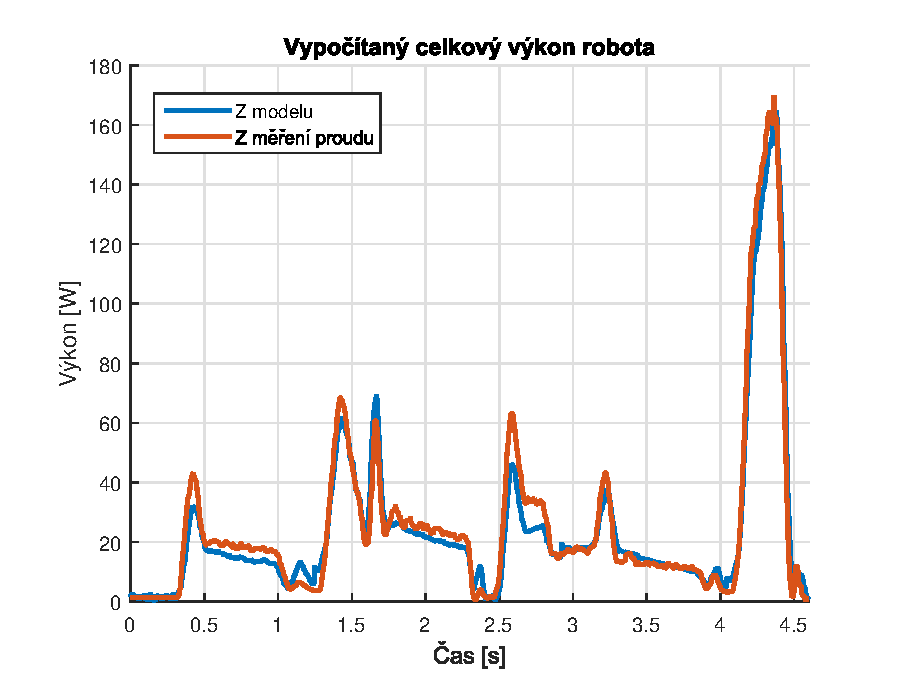
\includegraphics[width=0.90\textwidth]{model_vs_trace}
\caption{Srovnání vypočítaného výkonu z modelu a z měření proudu}
\label{model_vs_trace_pic}
\end{figure}

Na obrázku \ref{model_vs_trace_pic} je zobrazen průběh výkonu vypočítaného z modelu a z přímého měření proudů pomocí nástroje TRACE. Je patrné, že si oba průběhy poměrně odpovídají. Střední odchylka mezi oběma průběhy je 4,86 W. Přesnost odvozeného modelu se tedy blíží maximální možné dosažitelné přesnosti modelování a identifikace z rovnic.

\section{Reálný výkon}

